\documentclass[11pt,a4paper]{report}
\usepackage[portuges]{babel}
\usepackage[utf8]{inputenc} % define o encoding usado texto fonte (input)--usual "utf8" ou "latin1
\usepackage{graphicx} %permite incluir graficos, tabelas, figuras
\usepackage{subcaption}
\usepackage{listings}
\usepackage{color}
\usepackage{multicol}
\usepackage{indentfirst}
\usepackage{hyperref}
\usepackage{amsmath}
\usepackage{amssymb}
\usepackage{float}
\usepackage{enumitem}
\usepackage{tabularx}
\parskip=2pt % espaço entre o parágrafo e o texto anterior

\setlength{\oddsidemargin}{-1cm} %espaço entre o texto e a margem
\setlength{\textwidth}{18cm} %Comprimento do texto na pagina
\setlength{\headsep}{-1cm} %espaço entre o texto e o cabeçalho
\setlength{\textheight}{23cm} %altura do texto na pagina


\definecolor{myblue}{rgb}{0.2,0.2,0.8}
\definecolor{mygray}{rgb}{0.5,0.5,0.5}
\definecolor{mymauve}{rgb}{0.58,0,0.82}

\lstdefinestyle{code}{ 
  backgroundcolor=\color{white},   % choose the background color; you must add \usepackage{color} or \usepackage{xcolor}; should come as last argument
  basicstyle=\footnotesize,        % the size of the fonts that are used for the code
  breakatwhitespace=false,         % sets if automatic breaks should only happen at whitespace
  breaklines=true,                 % sets automatic line breaking
  captionpos=b,                    % sets the caption-position to bottom
  commentstyle=\color{white},    % comment style
  deletekeywords={...},            % if you want to delete keywords from the given language
  escapeinside={\%*}{*)},          % if you want to add LaTeX within your code
  extendedchars=true,              % lets you use non-ASCII characters; for 8-bits encodings only, does not work with UTF-8
  firstnumber=1000,                % start line enumeration with line 1
  keepspaces=true,                 % keeps spaces in text, useful for keeping indentation of code (possibly needs columns=flexible)
  keywordstyle=\color{blue},       % keyword style
  language=C++,                 % the language of the code
  morekeywords={*,...},            % if you want to add more keywords to the set
  numberstyle=\tiny\color{mygray}, % the style that is used for the line-numbers
  rulecolor=\color{black},         % if not set, the frame-color may be changed on line-breaks within not-black text (e.g. comments (green here))
  showspaces=false,                % show spaces everywhere adding particular underscores; it overrides 'showstringspaces'
  showstringspaces=false,          % underline spaces within strings only
  showtabs=false,                  % show tabs within strings adding particular underscores
  stepnumber=2,                    % the step between two line-numbers. If it's 1, each line will be numbered
  stringstyle=\color{mymauve},     % string literal style
  tabsize=2,	                   % sets default tabsize to 2 spaces
  title=\lstname                   % show the filename of files included with \lstinputlisting; also try caption instead of title
}

\title{Projeto - ComputationalMind\\ Desafios para Desenvolvimento  Computacional} %Titulo do documento

\author{Inês Pires Presa (A90355)\and Ivo Miguel Gomes Lima (A90214)\and Tiago André Oliveira Leite (A91694)\and Tiago dos Santos Silva Peixoto Carriço (A91695)} %autores do documento

\date{\today} %data

\begin{document}
	\begin{minipage}{0.9\linewidth}
        \centering
		
\includegraphics[width=0.4\textwidth]{um.jpeg}\par\vspace{1cm}
                \href{https://www.uminho.pt/PT}
		{\scshape\LARGE Universidade do Minho} \par
		\vspace{0.6cm}
                \href{https://lcc.di.uminho.pt}
		{\scshape\Large Licenciatura em Ciências da Computação} \par
		\maketitle
		\begin{center}
			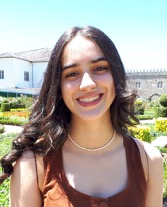
\includegraphics[width=0.24\linewidth]{ines.jpg}\hfill
			
\includegraphics[width=0.30\linewidth]{ivo.jpg}\hfill
			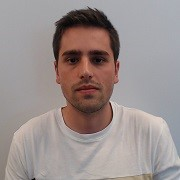
\includegraphics[width=0.30\linewidth]{tiago1.jpg}\hfill
			%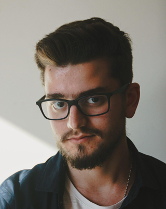
\includegraphics[width=0.24\linewidth]{tiago2.jpg}
		\end{center}
		
	\end{minipage}

\tableofcontents % insere Indice

\chapter{Introdução}

No âmbito da unidade curricular de Projeto da Licenciatura em Ciências da Computação, foi proposto o desenvolvimento de uma plataforma que permita inserir problemas/desafios para que os utilizadores possam, em modo jogo, responder a esses desafios. A plataforma deve ter uma interface de back-office (BO) para armazenar os problemas/desafios (nomeadamente o seu enunciado, opções de resposta, resposta certa, faixa etária, etc). 
A interface de front-office funciona em modo jogo para que os utilizadores possam responder aos desafios selecionados a partir do repositório criado no BO da plataforma. No modo jogo os utilizadores podem ter pontuações, prémios, ou outras formas de gamificação que os motivem e envolvam. \par
O presente relatório acompanha o processo de desenvolvimento do projeto.



\chapter{Enunciado do Projeto}

No âmbito do treino do Pensamento Computacional pretende-se criar uma plataforma que permita inserir proble-
mas/desafios para que os utilizadores possam, em modo jogo, responder a esses desafios. A plataforma deve ter
uma interface de back-office (BO) para armazenar os problemas/desafios (nomeadamente seu enunciado, opções de
resposta, resposta certa, faixa etária, etc). Um exemplo do tipo de exercicios que se pretende pode ser consultado
em: http://bebras.dcc.fc.up.pt/problems/2021/problemas\_09\_10.pdf
A interface de front-office funciona em modo jogo para que os utilizadores possam responder aos desafios
selecionados a partir do repositório criado no BO da plataforma. No modo jogo os utilizadores podem ter pontuações,
prémios, ou outras formas de gamificação que os motivem e envolvam.

\chapter{Mockups}

\begin{figure}[H]
\centering
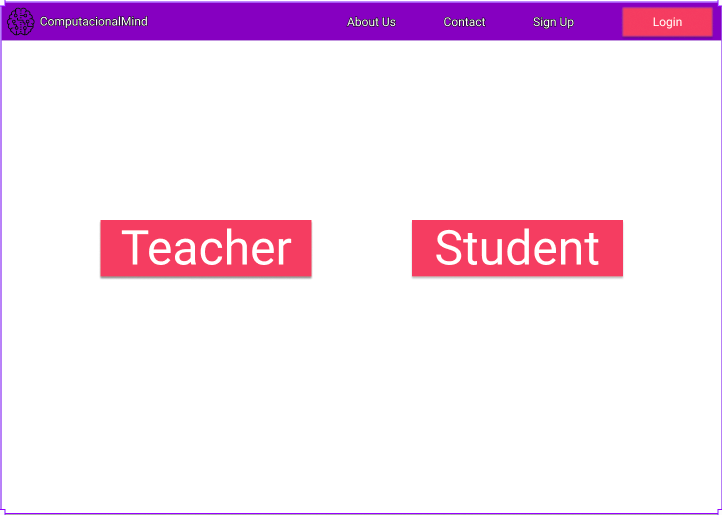
\includegraphics[width = 14cm,height = 10cm]{MockHome.png}
\caption{Página principal}
\label{fig:MockHome}
\end{figure}

\begin{figure}[H]
\centering
\includegraphics[width = 14cm,height = 10cm]{MockLogin.png}
\caption{Página de login}
\label{fig:MockLogin}
\end{figure}


\begin{figure}[H]
\centering
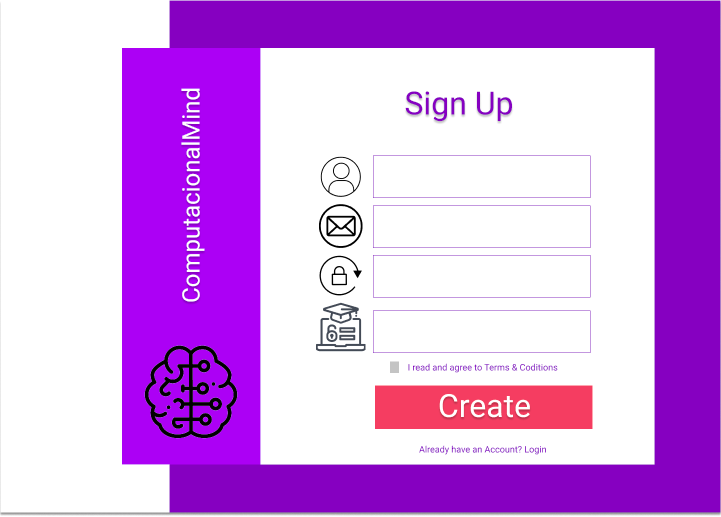
\includegraphics[width = 14cm,height = 10cm]{MockSingUp.png}
\caption{Página de criação de conta}
\label{fig:MockSingUp}
\end{figure}

\begin{figure}[H]
\centering
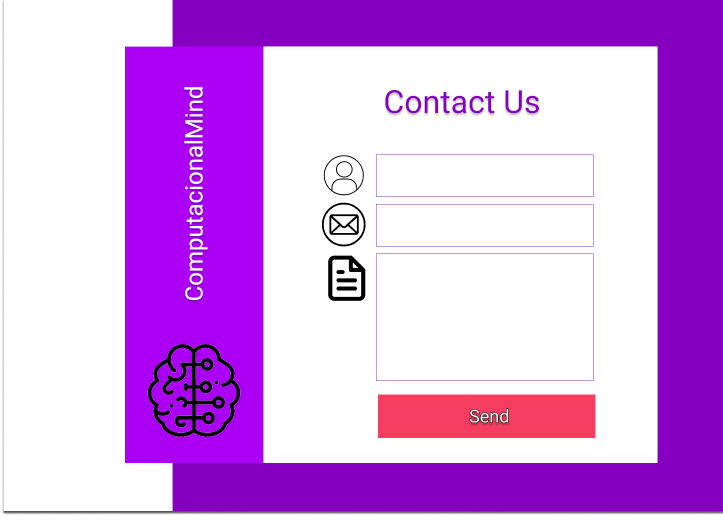
\includegraphics[width = 14cm,height = 10cm]{MockContactUs.png}
\caption{Página de contacto}
\label{fig:MockContactUs}
\end{figure}

\begin{figure}[H]
\centering
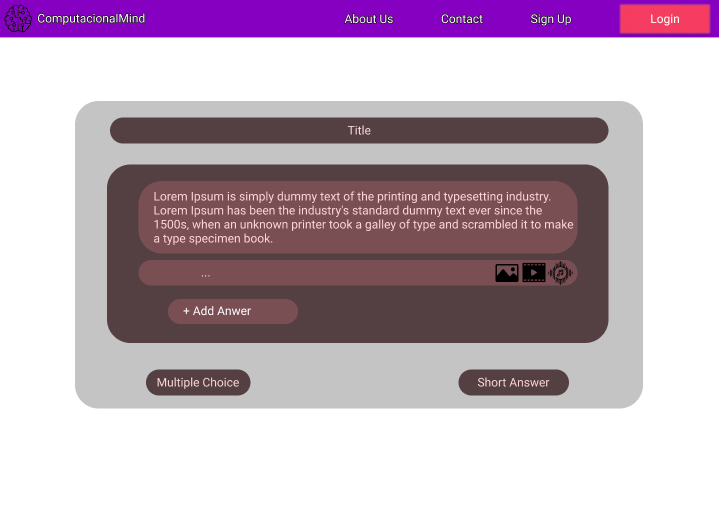
\includegraphics[width = 14cm,height = 10cm]{MockTeacherMenu.png}
\caption{Menu de inserção de jogo}
\label{fig:MockTeacherMenu}
\end{figure}


\begin{figure}[H]
\centering
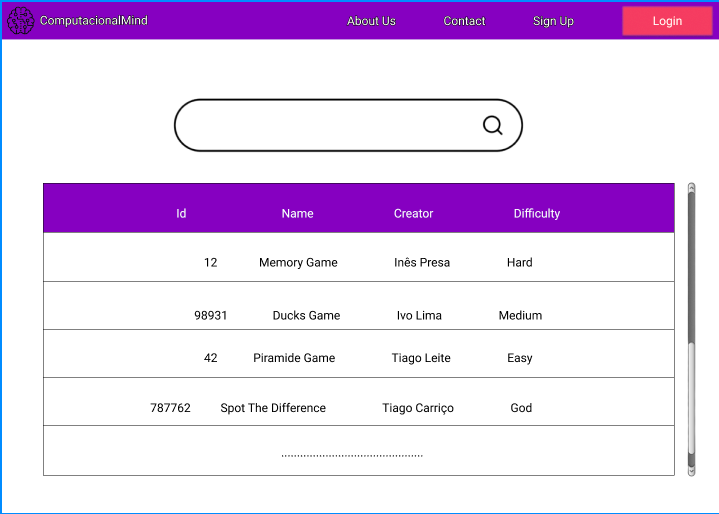
\includegraphics[width = 14cm,height = 10cm]{MockUserSelectGame.png}
\caption{Menu de selecção de jogo}
\label{fig:MockUserSelectGame}
\end{figure}

\begin{figure}[H]
\centering
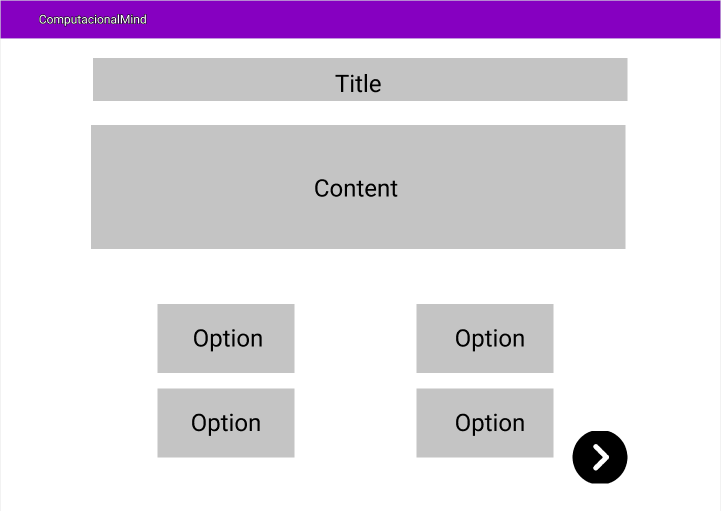
\includegraphics[width = 14cm,height = 10cm]{MockUserGameMC.png}
\caption{Jogo escolha múltipla}
\label{fig:MockUserGameMC}
\end{figure}

\begin{figure}[H]
\centering
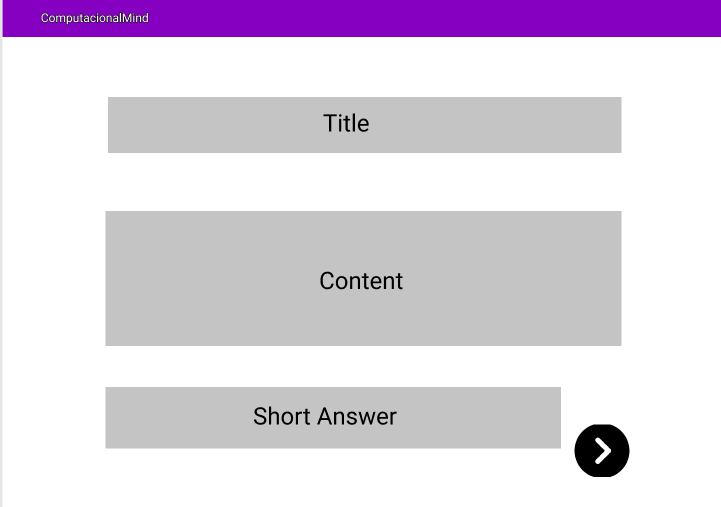
\includegraphics[width = 14cm,height = 10cm]{MockUserGameSA.png}
\caption{Jogo resposta curta}
\label{fig:MockUserGameSA}
\end{figure}

\begin{figure}[H]
\centering
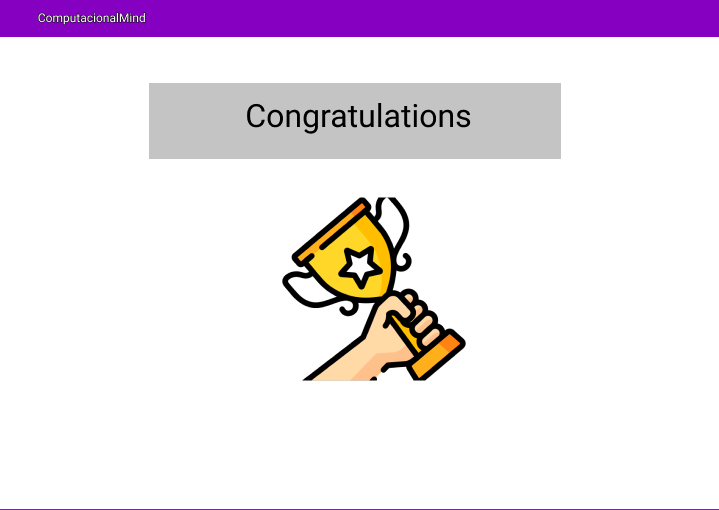
\includegraphics[width = 14cm,height = 10cm]{MockUserCongratulations.png}
\caption{Resposta certa}
\label{fig:MockUserCongratulations}
\end{figure}

\begin{figure}[H]
\centering
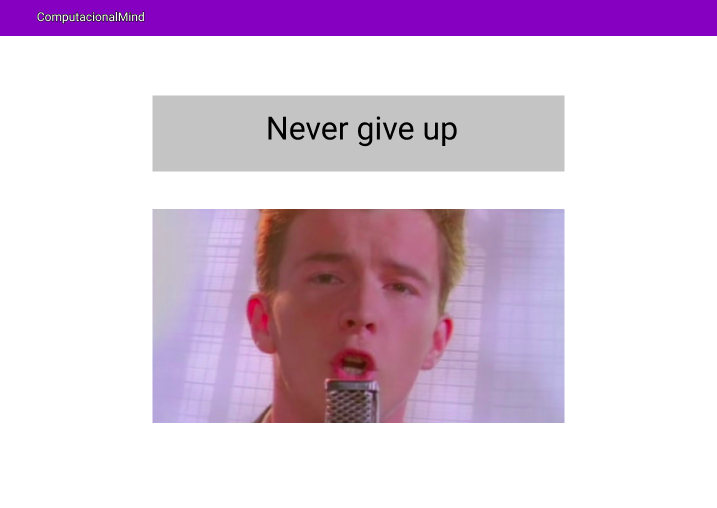
\includegraphics[width = 14cm,height = 10cm]{MockUserTryAgain.png}
\caption{Resposta errada}
\label{fig:MockUserTryAgain}
\end{figure}


\chapter{Base de Dados}

\section{Identificação e caracterização das entidades}

\subsection{Author}
Representa um autor que pode inserir jogos na plataforma.

\subsection{Player}
Representa um jogador da plataforma.

\subsection{Question}
Representa uma questão.

\subsection{Content}
Representa o conteúdo de uma questão.

\subsection{Option}
Representa uma opção de resposta para uma questão.

\subsection{History}
Representa o histórico de um jogador.

\section{Identificação e caracterização dos relacionamentos}

\begin{center}
\begin{tabular}{ |c|c|c|c|c| } 
 \hline
 \bf{Entidade} & \bf{Multiplicidade} & \bf{Relacionamento} & \bf{Multiplicidade} & \bf{Entidade} \\ 
 \hline
 Question & 1..N & tem & 1 & Author \\ 
 \hline
 Option & 1..N & tem & 1 & Question \\ 
 \hline
 History & 1..N & tem & 1 & Question \\ 
 \hline
 History & 1..N & tem & 1 & Player \\ 
 \hline
 Content & 1..N & tem & 1 & Question \\ 
 \hline
\end{tabular}
\end{center}

\section{Modelo Lógico}

\begin{figure}[H]
\centering
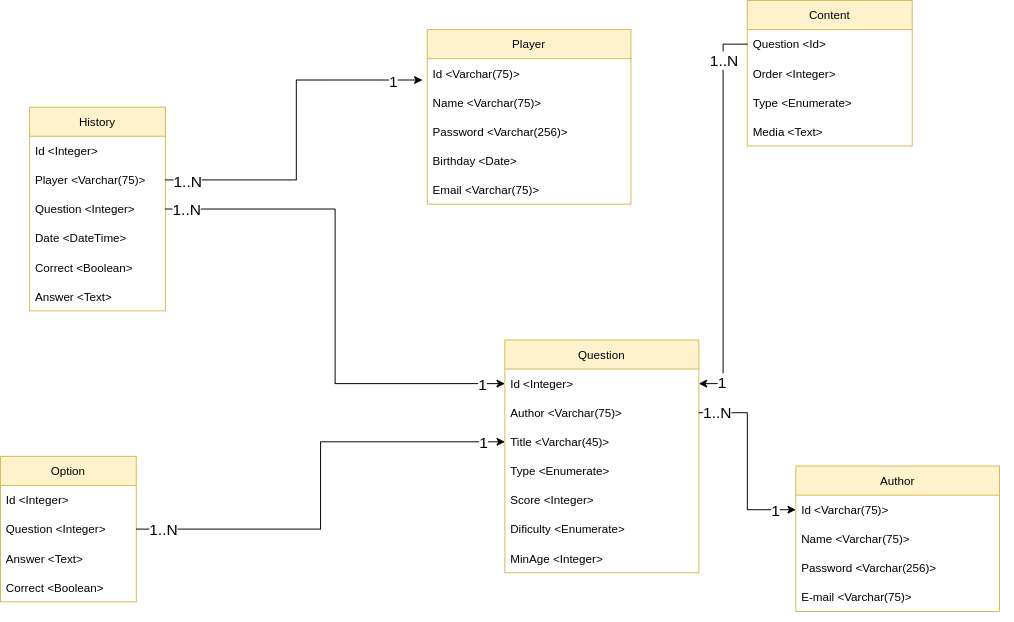
\includegraphics[width = 14cm,height = 10cm]{EsqLog.png}
\caption{Esquema Lógico}
\label{fig:EsqLog}
\end{figure}

\chapter{Conclusão}

\end{document}